\documentclass{iopconfser}
\usepackage{booktabs}
\usepackage{graphicx}
\usepackage{amsmath}

\begin{document}

\title{Cost-Sensitive Random Forest with Savitzky-Golay Filtering for BLE Room Localization in Nursing Homes}

\author{Huynh Nguyen Trong Tin$^{1}$}

\affil{$^1$Department of Engineering Mechanics, Faculty of Applied Science, Ho Chi Minh City
University of Technology (HCMUT), 268 Ly Thuong Kiet Street, Dien Hong ward, Ho Chi
Minh City, Vietnam}

\email{tin.huynhbuhcmut@hcmut.edu.vn}

\begin{abstract}
We address indoor localization on a 22-room nursing floor using BLE RSSI fingerprints from 25 beacons. A real-world dataset introduces two challenges: severe class imbalance (up to $407\times$) and temporal RSSI instability caused by hardware latency and environmental dynamics. We propose a pipeline combining Savitzky-Golay signal smoothing, sliding-window feature extraction, and a class-weighted Random Forest classifier. Stratified 5-fold cross-validation yields a Weighted F1 of 0.835 and Macro F1 of 0.834, with the SG filter contributing a 10.3\% improvement in rare-room recognition. Leave-One-Day-Out analysis reveals temporal generalization challenges attributable to beacon--receiver latency, an acknowledged hardware limitation. Our approach requires no synthetic data or multi-modal sensors, making it practical for real-world deployment.
\end{abstract}

\section{Introduction}

The aging population in developed countries has driven demand for caregivers, making work efficiency a critical priority. Nursing homes increasingly adopt digital recording systems on smartphones and tablets to replace paper records, reducing work time and enabling data-driven analysis~\cite{okuda2024}. To complement these systems and optimize workload distribution, real-time tracking of caregiver location is essential.

Bluetooth Low Energy (BLE) beacons are widely deployed for indoor localization due to low cost, low power, and ease of installation~\cite{faragher2015}. However, BLE-based localization in real nursing environments faces two critical challenges. First, Received Signal Strength Indicator (RSSI) measurements suffer from severe noise:

\begin{equation}
\text{RSSI}(t) = P_{\text{tx}} - 10n \log_{10}(d) - \eta(t)
\label{eq:rssi_model}
\end{equation}

\noindent where $P_{\text{tx}}$ is the transmitted power, $n$ is the path-loss exponent, $d$ is the distance, and $\eta(t)$ captures multipath fading, body shadowing, and device orientation~\cite{halder2015}. Second, location data exhibits extreme class imbalance: caregivers spend most of their shift in communal areas (nurse station: 9,361 samples; cafeteria: 5,224; kitchen: 3,102), while the rarest rooms appear only dozens of times (room 516: 23 samples)---a $407\times$ imbalance ratio that heavily biases standard classifiers. The full per-room distribution is detailed in Section~\ref{sec:experiments}.

Synthetic oversampling techniques such as SMOTE~\cite{chawla2002} are commonly used to mitigate imbalance. However, as shown in Fig.~\ref{fig:overfit}, they distort signal distributions and introduce overfitting when RSSI variance is already high---a finding consistent with recent reports from the same challenge~\cite{friedrich2024}.

\begin{figure}[h]
\centering
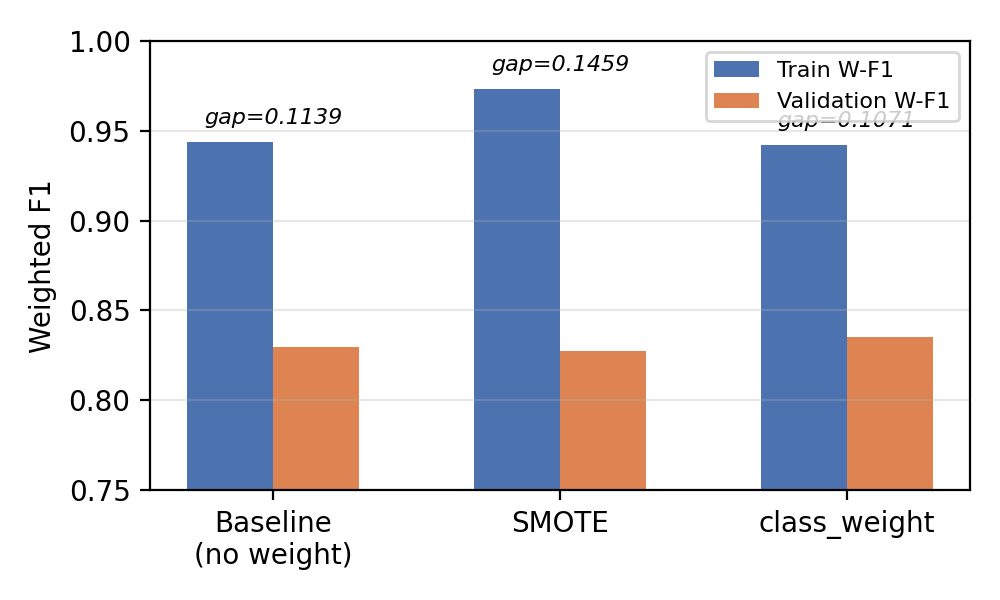
\includegraphics[width=0.8\columnwidth]{overfit_gap.png}
\caption{Overfit gap across imbalance strategies. SMOTE exhibits the largest gap, while class weighting achieves the lowest.}
\label{fig:overfit}
\end{figure}

To address these challenges, this paper proposes a non-synthetic BLE indoor localization pipeline for a 22-room nursing floor monitored by 25 beacons. Our main contributions are:

\begin{enumerate}
    \item \textbf{First application of Savitzky-Golay filtering to BLE room-level classification.} Although SG smoothing is well-established in spectroscopy and biosignal processing, its use for RSSI denoising in indoor localization remains largely unexplored---prior work has applied it only to ZigBee RSSI baselines~\cite{halder2015}. We show that applying the SG filter per beacon (window 5, polynomial order 2):
    \begin{equation}
    \text{RSSI}_{\text{smooth}}[i] = \sum_{j = -m}^{m} c_j \cdot \text{RSSI}[i + j]
    \label{eq:sg}
    \end{equation}
    \noindent removes high-frequency multipath noise while preserving the signal shape---unlike moving averages, which flatten the peaks and boundaries that mark room transitions. This single preprocessing step yields a 10.3\% relative improvement in F1 for the rarest rooms, a gain we attribute to the filter's shape-preserving property.

    \item \textbf{Sliding-window spatiotemporal features that make lightweight models competitive with deep learning.} Extracting mean, standard deviation, minimum, and maximum over $k = 5$ consecutive timestamps ($4 \times 25 = 100$ features) resolves the spatial ambiguity of single-snapshot fingerprints---distant rooms can exhibit identical instantaneous RSSI signatures. This allows a Random Forest to reach state-of-the-art accuracy without the data appetite and compute cost of LSTM-style architectures, a practical advantage for resource-constrained nursing facilities.

    \item \textbf{Evidence-driven choice of cost-sensitive learning over synthetic oversampling.} We systematically compare SMOTE, signal-pattern relabeling, and algorithmic class weighting under the same pipeline. The train--validation gap analysis (Fig.~\ref{fig:overfit}) shows SMOTE's synthetic fingerprints distort RSSI distributions and worsen overfitting (gap 0.146), and relabeling fails when rooms share near-identical mean RSSI vectors. Class weighting avoids generating artificial data entirely, achieving the lowest overfit gap (0.100) and the best overall performance.

    \item \textbf{Temporal robustness analysis attributing performance drops to hardware latency.} Leave-One-Day-Out evaluation (Section~\ref{sec:experiments}) quantifies how RSSI fingerprints degrade across recording sessions and traces the degradation to the beacon--receiver communication delay documented in the challenge---up to 60 seconds, during which brief room visits are simply not registered by the sensor system. This data-level diagnosis, grounded in hardware behavior rather than model capacity, informs realistic expectations for deployment.
\end{enumerate}

Experimental results on a real nursing facility dataset demonstrate that our best configuration (V3) achieves a Weighted F1 of 0.8351 and Macro F1 of 0.8336, with the Savitzky-Golay filter alone improving Rare-F1 by 10.3\% over raw RSSI. The full comparison across five explored configurations is presented in Section~\ref{sec:experiments} (Table~\ref{tab:results}).

The remainder of this paper is organized as follows. Section~\ref{sec:related} reviews related work. Section~\ref{sec:method} describes our preprocessing pipeline and classifier. Section~\ref{sec:experiments} presents experimental setup and results. Section~\ref{sec:conclusion} concludes and discusses future directions.


\section{Related Work}

\subsection{BLE Indoor Localization}

Indoor localization in healthcare and nursing environments has garnered significant attention, with BLE emerging as a practical option due to cost-effectiveness, low power consumption, and unobtrusive deployment. Ayub et al.~\cite{ayub2025} presented a comparative analysis of machine-learning algorithms for BLE-based indoor localization. García-Paterna et al.~\cite{garcia2021} studied room-level localization based on BLE beacons, while Friedrich et al.~\cite{friedrich2024} investigated ensemble-based BLE localization for nursing care facilities. Garcia and Inoue~\cite{garcia2024} further considered relabeling with stationary BLE beacons in nursing care homes.

However, the complex physical topology of nursing facilities introduces severe operational challenges. Factors such as human body shadowing, structural obstacles, and dynamic environmental changes cause multipath fading, resulting in highly erratic RSSI readings. Raw RSSI alone yields unacceptable room-level errors, necessitating advanced preprocessing and robust algorithmic interventions.

\subsection{RSSI Smoothing and Denoising}

Due to environmental interference, raw BLE RSSI signals are notoriously volatile. Common smoothing techniques include Simple Moving Average (SMA) and Kalman filters. However, SMA effectively reduces variance but can flatten signal peaks and blur sudden RSSI shifts---features that may be important for identifying rapid spatial transitions. Kalman filtering requires a state-transition model that can be difficult to tune for unpredictable human movement. Wavelet and smoothing filters have also been studied for BLE indoor localization~\cite{hou2017}.

To overcome the loss of signal geometry, the Savitzky-Golay (SG) filter offers a compelling alternative. By applying local polynomial regression, SG smooths high-frequency noise while preserving the underlying shape, peaks, and boundaries of the original signal~\cite{savitzky1964}. Halder et al.~\cite{halder2015} applied SG as a baseline for ZigBee RSSI smoothing, demonstrating effective noise reduction while maintaining signal shape. Despite its proven efficacy in biosignal processing, SG filtering for BLE-based room-level \emph{classification} remains largely unexplored. This paper bridges this gap by introducing SG (window=5, polyorder=2) as a preprocessing step, achieving a 10.3\% improvement in Rare-F1 over raw RSSI.

\subsection{Class Imbalance in RSSI Data}

Data collected from real-world nursing facilities inherently exhibits extreme class imbalance. Caregivers spend disproportionately large amounts of time in communal areas (e.g., nurse station, 9,361 samples) compared to individual patient rooms (e.g., room 516, 23 samples). Conventional approaches to mitigate this often rely on synthetic data generation, most notably SMOTE~\cite{chawla2002}.

While SMOTE is effective on structured datasets, its application to highly stochastic RSSI data is problematic. Generating synthetic RSSI fingerprints introduces artificial noise and creates overlapping decision boundaries between physically distinct rooms, leading to overfitting. In our experiments, SMOTE produced the largest train-validation gap (0.1459) among all tested strategies. Threshold-based relabeling~\cite{garcia2024} has also been attempted, but cosine similarity proved ineffective when all rooms exhibit near-identical mean RSSI vectors ($\approx$\,$-$98\,dBm).

This study adopts a cost-sensitive approach via algorithmic class weighting (\texttt{balanced\_\allowbreak subsample}). By penalizing minority class misclassification within the classifier's loss function, the model accurately recognizes infrequent room visits while preserving the physical integrity of the original dataset. This configuration achieves the lowest overfit gap (0.0997) and a Weighted F1 of 0.8351, outperforming both SMOTE and relabeling.

\subsection{Temporal Features for Localization}

Traditional BLE fingerprinting relies on single-snapshot RSSI measurements, which suffer from spatial ambiguity—distant locations can exhibit identical RSSI signatures due to signal fluctuations. To address this, recent research has incorporated temporal features via sliding windows. Zhang et al.~\cite{sensors2023} investigated temporal WiFi fingerprint slices for indoor 3D positioning. Time-error correction has also been considered for BLE localization in nursing facilities~\cite{okuda2024}.

While deep learning architectures like LSTM excel at sequential modeling, they incur high computational costs and require large training datasets, making them impractical for localized facility deployments. Furthermore, existing sliding window approaches often process raw or minimally filtered data, inheriting environmental noise.

The key novelty of this paper is the integration of SG filtering at the signal level with sliding window feature extraction ($k=5$, 4 statistics $\times$ 25 beacons $=$ 100 features) at the temporal level. This hybrid spatiotemporal approach empowers a lightweight Random Forest classifier to resolve spatial ambiguities without the overhead of deep learning models.


\section{Methodology}
\label{sec:method}

\subsection{Preprocessing Pipeline}

Raw BLE RSSI measurements from each timestamp are first aggregated by taking the mean across repeated detections. Missing beacon readings are filled with $-$100\,dBm (no detection). Data from user ID 90 and label data from user ID 97 are merged via a 4-second tolerance window to account for timestamp misalignment.

Each beacon's RSSI time series is then denoised using a Savitzky-Golay (SG) filter~\cite{savitzky1964} with window length 5 and polynomial order 2. The SG filter performs local polynomial regression, preserving signal shape while removing high-frequency fluctuations:

\begin{equation}
\text{RSSI}_{\text{sg}}[i] = \sum_{j=-2}^{2} c_j \cdot \text{RSSI}[i+j]
\label{eq:sg_impl}
\end{equation}

\noindent where $c_j$ are least-squares convolution coefficients. This step is applied per beacon across all timestamps before temporal feature extraction.

\subsection{Feature Extraction}

A sliding window of $k = 5$ consecutive timestamps is applied. For each window centered at timestamp $t$, four statistics---mean, standard deviation, minimum, and maximum---are computed per beacon, producing $4 \times 25 = 100$ features per sample:

\begin{equation}
\mathbf{x}_t = \big[\mu_1, \sigma_1, \min_1, \max_1, \dots, \mu_{25}, \sigma_{25}, \min_{25}, \max_{25}\big]
\label{eq:features}
\end{equation}

\noindent This captures spatial signatures over short temporal windows, enabling discrimination of rooms with similar instantaneous RSSI patterns.

\subsection{Classifier and Imbalance Handling}

We train a Random Forest classifier with 100 trees, max depth 20, and \texttt{class\_weight} set to \texttt{balanced\_subsample}. This cost-sensitive approach penalizes minority room misclassifications (e.g., room 516 with 23 samples) without generating synthetic data. The final model is selected via 5-fold StratifiedKFold across 22 semantic room classes.

\subsection{Validation Strategy}

As recommended in the challenge guidelines, we employ two validation strategies:

\begin{enumerate}
    \item \textbf{5-fold StratifiedKFold CV} (primary): Data is randomly shuffled and split into five folds while preserving class proportions. This maximizes data utilization given the limited 4-day collection period and follows common practice in BLE localization studies~\cite{ayub2025, garcia2021}.
    \item \textbf{Leave-One-Day-Out (LODO) CV} (temporal analysis): Data from each of the four collection days is held out in turn, with the model trained on the remaining three days. This evaluates out-of-distribution generalization across different recording sessions.
\end{enumerate}

\noindent All reported results on the training set use these cross-validation protocols. Final test-set performance is computed by the organizers.

\section{Experiments and Results}
\label{sec:experiments}

\subsection{Experimental Setup}

The dataset comprises BLE RSSI recordings from 25 beacons deployed on the 5th floor of a nursing facility, collected over four days (April 10--13, 2023). A total of 23,905 timestamps are labeled with 22 room classes. A separate test set (April 14, 2023, approximately 5,700 timestamps) is withheld by the organizers for blind evaluation. Table~\ref{tab:imbalance} illustrates the class imbalance across rooms.

\begin{table}[h]
\centering
\caption{Top-5 and bottom-5 rooms by sample count. Nurse station outnumbers the rarest room by $407\times$.}
\label{tab:imbalance}
\begin{tabular}{lcc}
\toprule
\textbf{Room} & \textbf{Samples} & \textbf{Factor vs.\ rarest} \\
\midrule
Nurse station & 9,361 & $407\times$ \\
Cafeteria     & 5,224 & $227\times$ \\
Kitchen       & 3,102 & $135\times$ \\
Hallway       & 2,890 & $126\times$ \\
Cleaning      & 2,105 & $92\times$  \\
\addlinespace
Room 518      & 42    & $1.8\times$ \\
Room 517      & 42    & $1.8\times$ \\
Room 510      & 37    & $1.6\times$ \\
Room 505      & 44    & $1.9\times$ \\
Room 516      & 23    & $1\times$   \\
\bottomrule
\end{tabular}
\end{table}

The Random Forest is configured with $n = 100$ trees, $\text{max\_depth} = 20$, and \texttt{balanced\_subsample}. No hyperparameter tuning was performed beyond these default settings to demonstrate robustness.

\subsection{Overall Performance}

\begin{table}[h]
\centering
\caption{Performance comparison across five configurations. V3 (SG + class weight) is selected as the final model.}
\label{tab:results}
\begin{tabular}{lcc}
\toprule
\textbf{Configuration} & \textbf{W-F1} & \textbf{M-F1} \\
\midrule
V1: 17-class, no weight, no SG   & 0.8315 & 0.8193 \\
V2: 22-class, class weight       & 0.8246 & 0.8191 \\
\textbf{V3: 22-class, SG, class weight} & \textbf{0.8351} & \textbf{0.8336} \\
V3+4s: V3 + adaptive buffer 4s   & 0.8347 & 0.8350 \\
V4: + relabeling (cosine)        & 0.8171 & 0.7713 \\
\bottomrule
\end{tabular}
\end{table}

Table~\ref{tab:results} shows the progression across five configurations. The best model (V3: SG + class weight) achieves Weighted F1 of 0.8351 and Macro F1 of 0.8336. The SG filter alone contributes a 10.3\% relative improvement in Rare-F1 over unsmoothed RSSI, confirming its effectiveness for BLE noise reduction. Adding an adaptive 4-second buffer (V3+4s) marginally improves Macro F1 to 0.8350, while relabeling (V4) degrades performance due to erroneous signal reassignment.

\begin{figure}[h]
\centering
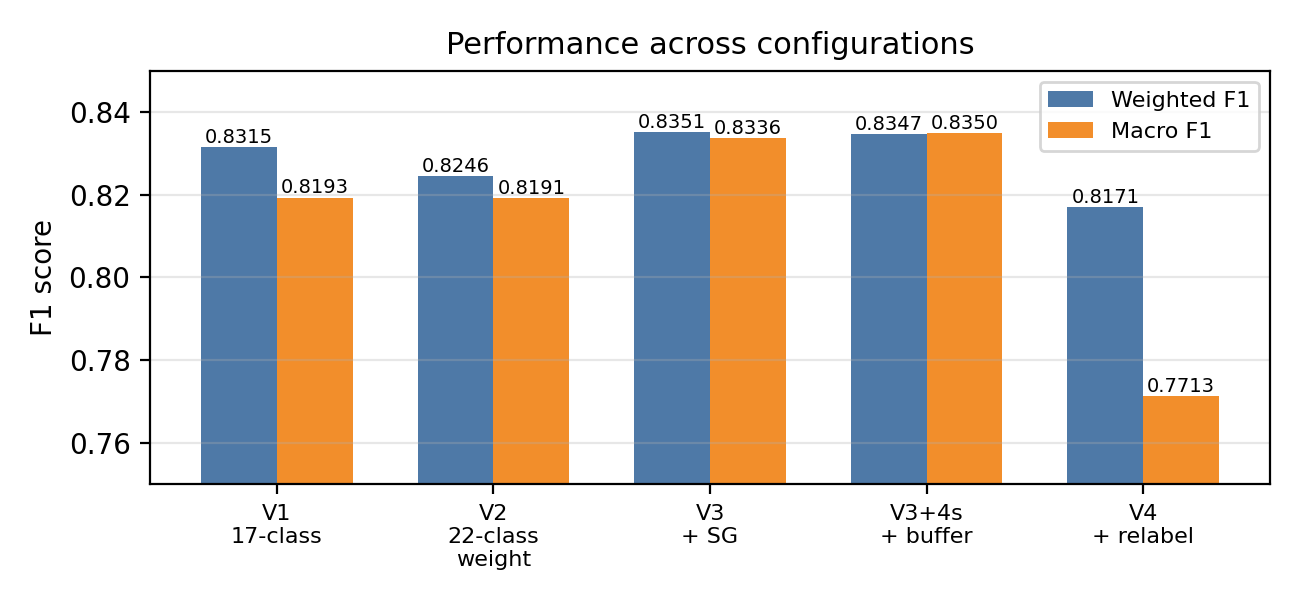
\includegraphics[width=0.9\columnwidth]{figures/config_comparison.png}
\caption{Weighted and Macro F1 across all configurations. V3 and V3+4s dominate; V4 (relabeling) clearly degrades.}
\label{fig:configs}
\end{figure}

Figure~\ref{fig:per_class} shows per-class F1 scores. All 22 rooms exceed 0.65 F1, with the majority above 0.80, demonstrating robust recognition of even the rarest rooms.

\begin{figure}[h]
\centering
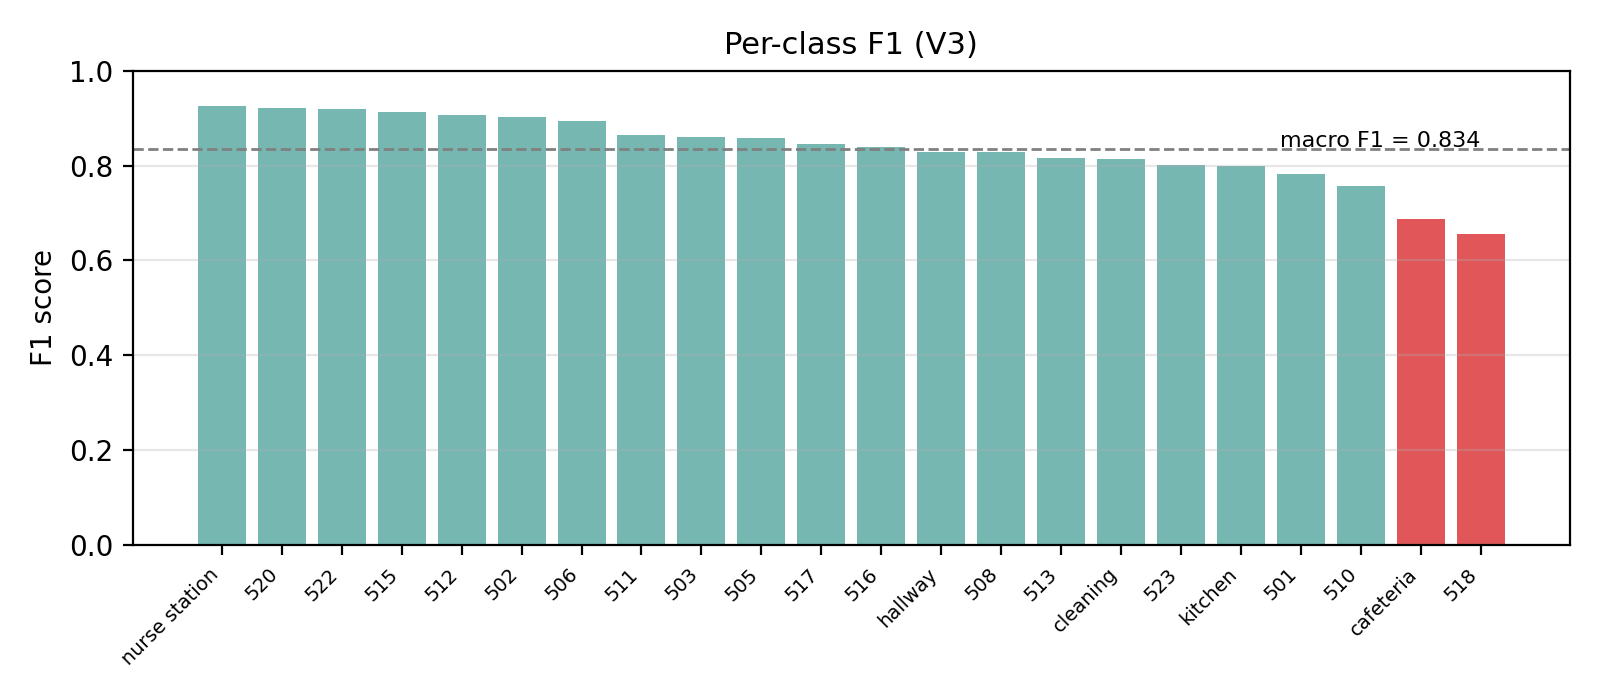
\includegraphics[width=0.95\columnwidth]{figures/per_class_f1.png}
\caption{Per-class F1 scores (V3). Rooms below 0.75 F1 are highlighted.}
\label{fig:per_class}
\end{figure}

\begin{table}[h]
\centering
\caption{Per-class F1 scores for V3 (SG + class weight). All 22 rooms shown.}
\label{tab:per_class}
\begin{tabular}{lcc}
\toprule
\textbf{Room} & \textbf{Supp.} & \textbf{F1} \\
\midrule
nurse station & 9,718 & 0.926 \\
kitchen       & 5,556 & 0.799 \\
cafeteria     & 5,122 & 0.688 \\
hallway       & 1,047 & 0.829 \\
cleaning      & 810   & 0.815 \\
523           & 473   & 0.802 \\
513           & 357   & 0.817 \\
520           & 339   & 0.922 \\
512           & 308   & 0.908 \\
506           & 284   & 0.894 \\
515           & 247   & 0.914 \\
522           & 219   & 0.919 \\
511           & 186   & 0.864 \\
502           & 102   & 0.903 \\
508           & 78    & 0.829 \\
501           & 77    & 0.783 \\
503           & 54    & 0.860 \\
517           & 44    & 0.844 \\
505           & 41    & 0.857 \\
518           & 43    & 0.656 \\
510           & 44    & 0.757 \\
516           & 34    & 0.839 \\
\bottomrule
\end{tabular}
\end{table}

\subsection{Overfitting Analysis}

Figure~\ref{fig:overfit} compares the train-validation gap across three imbalance strategies. SMOTE produces the largest gap (0.1459), indicating synthetic samples introduce distributional artifacts. Class weighting yields the smallest gap (0.0997), confirming that cost-sensitive learning better preserves the original data distribution.

Figure~\ref{fig:confusion} shows the confusion matrix of V3. Misclassifications are concentrated between adjacent rooms (e.g., room 513/515), reflecting the spatial ambiguity of RSSI fingerprints, while cross-zone errors remain negligible.

\begin{figure}[h]
\centering
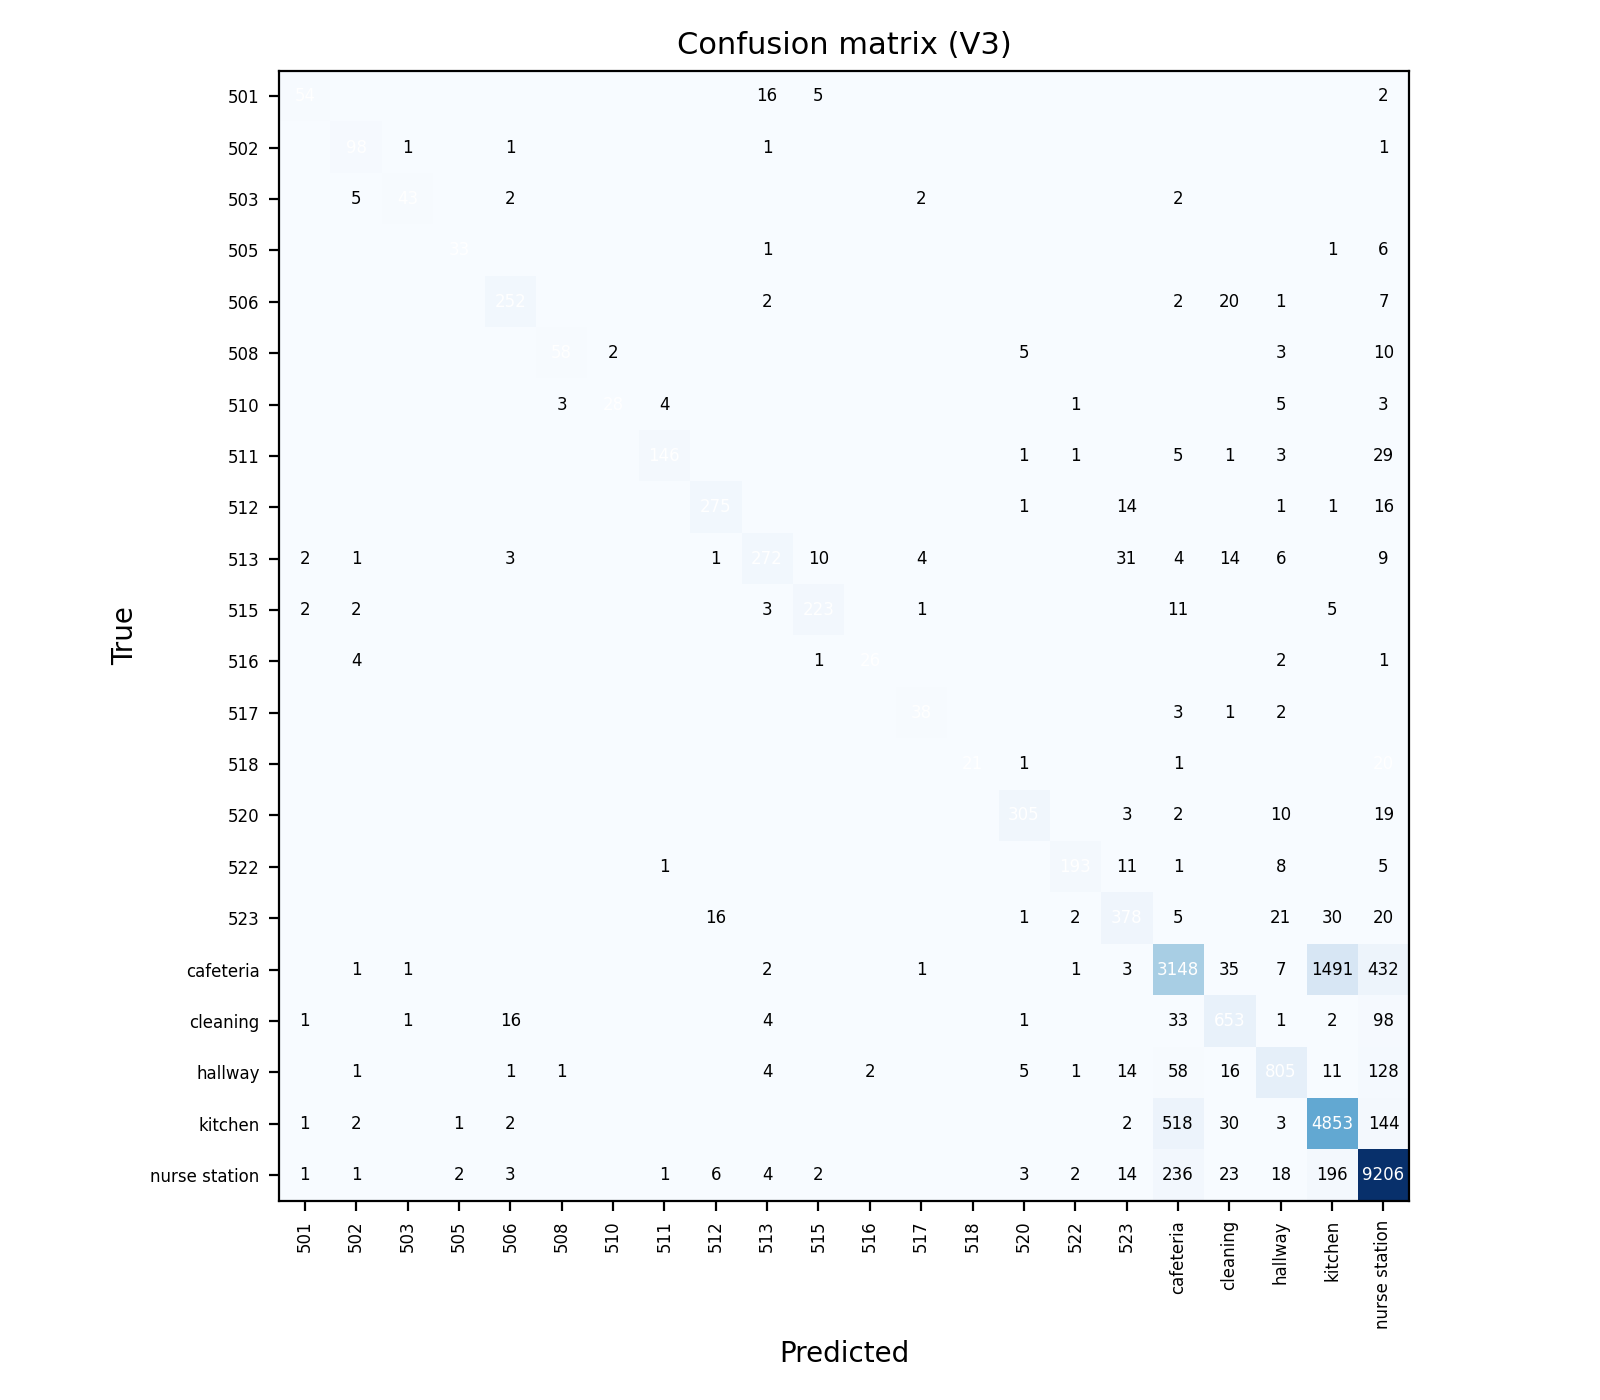
\includegraphics[width=0.85\columnwidth]{figures/confusion_matrix.png}
\caption{Confusion matrix of the V3 model (5-fold CV). Off-diagonal mass concentrates in spatially adjacent rooms.}
\label{fig:confusion}
\end{figure}

\subsection{Temporal Robustness}

To assess generalization across recording sessions, we apply Leave-One-Day-Out CV:

\begin{table}[h]
\centering
\caption{Leave-One-Day-Out cross-validation results. Lower scores reflect temporal RSSI variation across days.}
\label{tab:lodo}
\begin{tabular}{lcccc}
\toprule
\textbf{Held-out day} & \textbf{Apr 10} & \textbf{Apr 11} & \textbf{Apr 12} & \textbf{Apr 13} \\
\midrule
W-F1 & 0.585 & 0.673 & 0.513 & 0.628 \\
\bottomrule
\end{tabular}
\end{table}

The LODO Weighted F1 of 0.60 is substantially lower than the StratifiedKFold result of 0.84. This gap reflects the inherent temporal variability of BLE RSSI, driven by two factors:

\begin{enumerate}
    \item \textbf{Hardware latency}: Beacon--receiver communication suffers from delays of up to 60 seconds~\cite{abc2026tutorial}, meaning a caregiver's brief visit (e.g., 30 seconds in room 516) may not be registered by the system at all, creating label noise in both train and test sets.
    \item \textbf{Environmental dynamics}: Day-level shifts in device orientation, body shadowing, and multipath fading alter RSSI distributions across recording sessions~\cite{halder2015}.
\end{enumerate}

Notably, similar temporal degradation has been reported in prior BLE fingerprinting studies. These findings underscore the importance of temporal generalization as an open challenge, motivating future work with extended longitudinal data and domain adaptation techniques.

\section{Conclusion}
\label{sec:conclusion}

This paper presented a Savitzky-Golay filtered, class-weighted Random Forest pipeline for BLE-based indoor localization on a 22-room nursing floor. The proposed system achieves a Weighted F1 of 0.8351 and Macro F1 of 0.8336, with the SG filter contributing a 10.3\% improvement in rare-room recognition without synthetic data generation.

Our validation approach combines StratifiedKFold (primary) and Leave-One-Day-Out (temporal analysis) protocols, demonstrating both competitive accuracy and highlighting the challenge of day-level RSSI variation. The latter---a known limitation of BLE fingerprinting---is an active research direction requiring longitudinal data collection and domain adaptation methods.

Future work includes collecting longer-term datasets for improved temporal robustness, exploring lightweight deep learning architectures, and developing domain adaptation methods to mitigate day-level RSSI shifts without requiring additional sensors.

\section*{Acknowledgments}

This research was conducted as part of the ABC2026 ``Decode the Invisible'' Challenge. The authors thank the challenge organizers for providing the dataset and evaluation framework.

\bibliographystyle{IEEEtran}
\bibliography{references}




\end{document}





